\section{Model Generation}
The main goal of the present work, as stated before, is to recreate a three-dimensional virtual model of histological tissue as faithfully as possible and then, to perform a planar sectioning on it to emulate virtually the traditional histological specimen preparation procedure. The creation of a model of such complex structures is definetly an high-level problem, and it has required a carefull designing, made of successive phase of improvements. In this work I will report only two specific attempts of modelization: the first aiming to report pancreatic tissue, and the second oriented toward dermatic tissue.

\begin{figure}[b!]
    \centering
    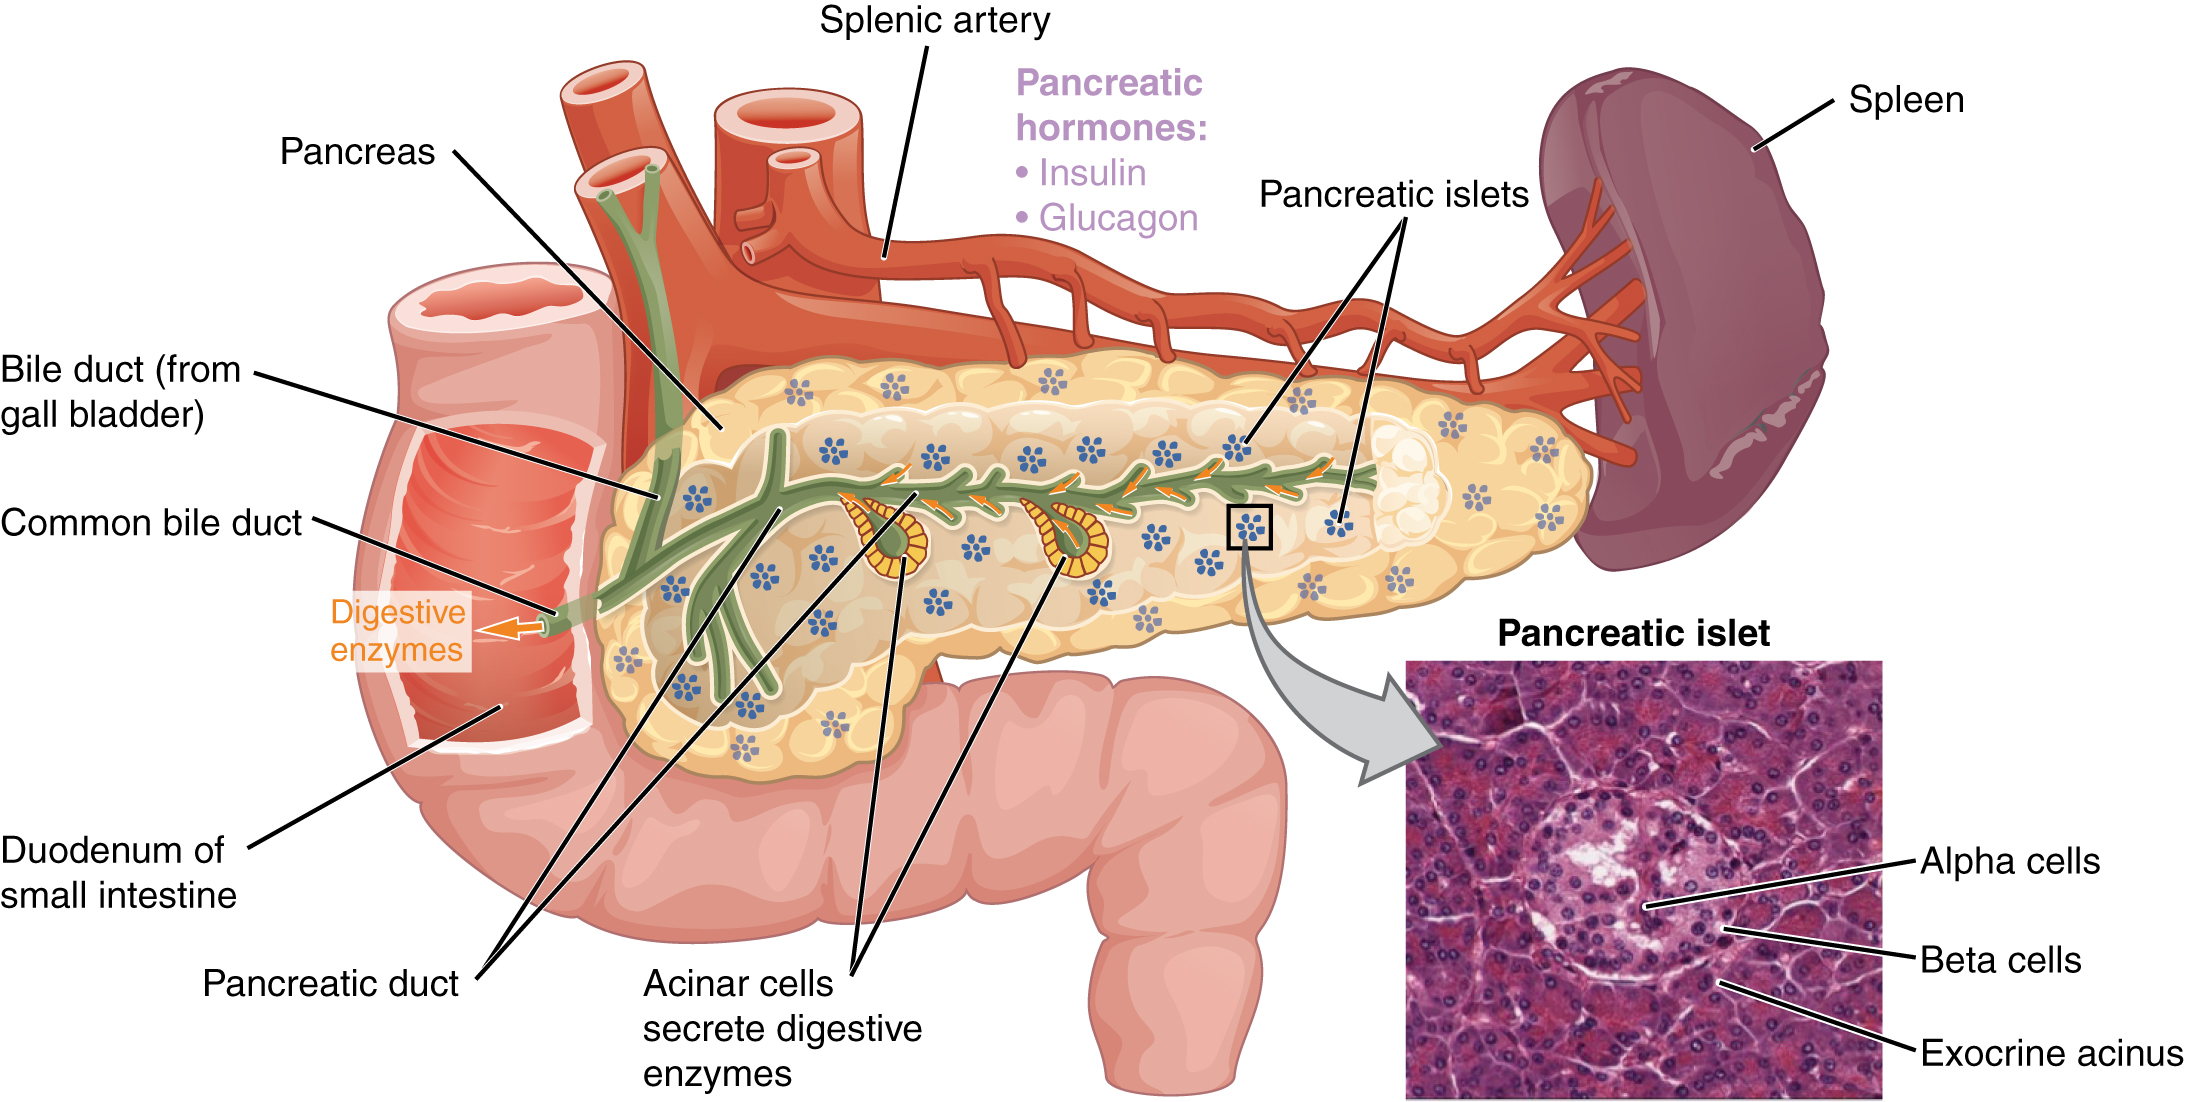
\includegraphics[width = 0.6\textwidth]{images/panc_struct}
    \caption{A picture of pancreas' structure in its phisiologiacl context. In this picture is clearly visible the macroscopic structure and the galndular organization at microscopic level, and how it reflects in the histological sample.}
    \label{fig:panc_struct}
\end{figure}

\subsection{Pancreas Tissue Model} \label{ssec:panc_tis_mod}
The Pancreas is an internal organ of the human body, part of both the digestive system and endocrine system. It acts as a gland with both endocrine and exocrine functions, and it is located in the abdomen behind the stomach. Its main endocrine duty is the regulation of sugar levels in blood and the secretion of hormones, as insulin, glucagon. While, as a part of the digestive system it acts as an exocrine gland secreting pancreatic juice. The majority of pancreatic tissue has a digestive role, and the cells with this role form clusters (\textit{acini}) around the small pancreatic ducts, and are arranged in lobes. The acinus secrete inactive digestive enzymes called zymogens into the small intercalated ducts which they surround, and then in the pancreatic blood vessels system \cite{Pancreas}. In Figure \ref{fig:panc_struct} is reported a picture of pancreas, with its structure and its placement in the human body.

All the tissue is actually rich of others important elements as the islets of Langerhans, and sporadic connective tissue allover the structure, which are clearly visible in the traditional histological specimens. In this first attempt of modelization from scratch this second layer of complexity has not been already considered, and the main focus was to reflect only the main structural features on the virtual specimen. Given pancreatic tissue's organization the first features I decided to put emphasis on were: 1) The iterative (with a fractal-like behavior) ramification of blood vassels for the irroration of glandular acinus, 2) The space-filling distribution of acinus in the tissue, in fact we expect an homogeneous density in the organ and to not see \textit{holes} at all inside it. In this secton I will describe step by step all the process I followed to create the model of a portion of pancreatic tissue, and all the interesting pitfalls I overcame.

\hl{[Should I make a bullet point list here? or going along with the text's flux?]}

The first step was took in 2 dimensions, and it was the choice of the right \textit{structure} to emulate the ramification of blood vessels in pancreatic tissue. The choice fell on a particular parametric L-system, as the one shown in Figure \ref{fig:bf_ls}, in section \ref{sec:tech_tool}. This structure is made of an iterative bifurcation of gradually shorter segments, with an angle of $\pm 85 \degree$ respect the main direction. For a start I added some features to give a more realistic look to the structure, which are all well represented in Figure \ref{fig:ram_feat}:

\begin{figure}
    \centering
    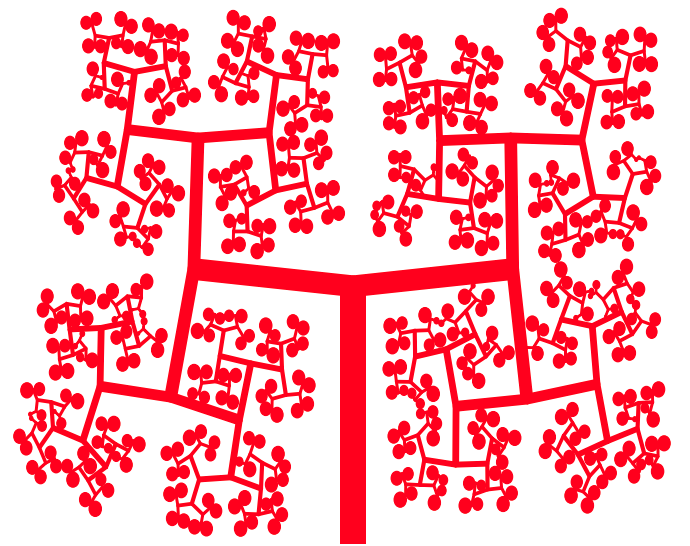
\includegraphics[width = 0.6\textwidth]{images/ram_feat}
    \caption{The development of the simple curve in Figure \ref{fig:bf_ls}, with some features to give it a more realistic look, like progressive thickness, angular noise in bifurcation and spheres at free ends of the ramification. The image is made using the tools exposed in section \ref{ssec:Lsys}.}
    \label{fig:ram_feat}
\end{figure}

\begin{itemize}
    \item A pregressive thickness of the bifurcation's segments, starting from a thick main branch which dwindle every junction. The idea is that the main blood vessel becomes via via smaller becoming capillars for a single cell irroration.
    \item A progressive randomness in the angular deflection at every fork. Perfectly repeated angles are almost nonexistent in nature, so I decided to introduce an increasing indetermination in the angle of bifurcation from the main branch to the free ends of the structure'branches.
    \item Spheres at the ends of each branch, which acts as glandular acini. The maximum radius is comparable to the length of final segments.
    \item A mechanism to avoid self-superimposition between branches and spheres. After the insertion of noise, the cumulative effect on the final segments might lead different branches to intersect. This is crearly a paradoxal situation, as real tissues while growing naturally occupy the space in a gradual way.
\end{itemize}

To produce the specific image in Figure \ref{fig:ram_feat} I used a prticular setting of the tools described in section \ref{ssec:Lsys}, which have a greatly wider range of customization, and could be used to create many other different structures.

The successive step I followed was to expand this structure in three dimensions, and fill the space in each of the three directions. The idea to evolve the structure in Figure \ref{fig:ram_feat} is simply to twist of 90$\degree$ the ramification at every junction point, in such a way to exit the previous plane. However, putting into practice this development has not been easy. The organization of the structure in a 3D space requires an appropriate system of reference for handling subsequent rotations in three dimensions. The best option for handling relative 3D rotations, often used in computer graphics and in every kind of 3D modelization, are quaternions, as shown in \ref{ssec:quat}.

\begin{figure}
    \centering
    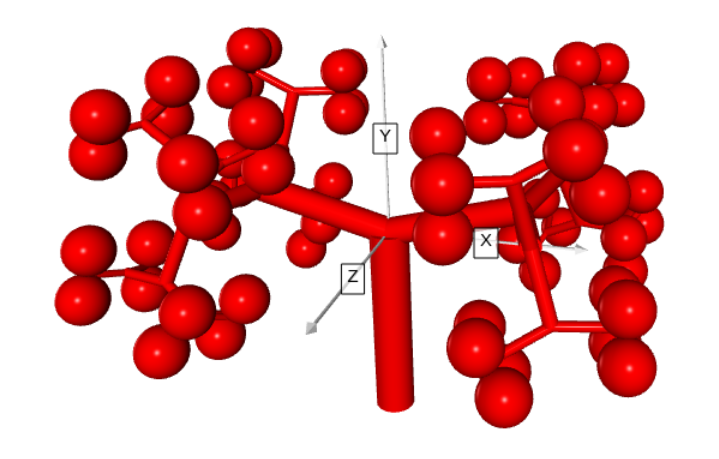
\includegraphics[width = 0.6\textwidth]{images/3d_ram}
    \caption{The three-dimensional expansion of the 2D ramification in Figure \ref{fig:ram_feat}.}
    \label{fig:3d_ram}
\end{figure}

In this new structure segments are replaced with cylinders, and circles are replaced with spheres. At each bifurcation to every cylinder corresponds:
\begin{itemize}
    \item a contraction in its extensions, regulated by an adjustable parameter $R$.
    \item the usual deviation of $\pm 85 \degree$ respect to the direction of the parent branch.
    \item a 90$\degree$ specific rotation along the axis of its parent branch.
\end{itemize}

The result of this procedure is a 3D ramification like the one in Figure \ref{fig:3d_ram}, in which we can recognise a good coverage of the space defined by the structure's boundaries and an immediate relation with the 2D structure in Figure \ref{fig:ram_feat}. It should be noted that, in the further refinments of the model from now on, there won't be present the progressive angular indetermination on the direction of branches. Altough it is a feature already implemented and working, it requires an efficient control for avoid reciprocal overlapping between elements to produce a realistic structure. This second element has not been already developed and it would certainly enrich the representative power of the model.

As for the 2D ramification the production of this structure has required the implementation of a tool for 3D generation of greatly wider power, able to produce almost any type of three-dimensional iterative structure after the right adjustment, and with an high degree of customization. It is necessary to mention the foundamental tool which allowed me to accomplish this step of the devolpment, which is the \texttt{Python} library \texttt{VPython}: a library for 3D graphics visualization for python. This library allows a convinient and powerfull interface to draw many types of objects and to move them around in space, which has been priceless to orient my self in three dimensions while developing the model, and to produce all the 3D images visible in this work.
\\
VORONOI AS CELLS\\
CHOICE OF SEMIRANDOM POINTS\\
IDETITY ASSIGMENT TO CELLS\\
SECTIONING AND IMAGE PRODUCTION -> SEGMENTATION MASK\\
\\
ADJUSTMENTS: PALETTE, NOISE, STYLE TRANSFER\\
\\
PIPELINE TO AUTOMATIZATION\\
\clearpage
